\documentclass[journal]{IEEEtran}
\IEEEoverridecommandlockouts

%% ---- Packages ----
\usepackage[T1]{fontenc}
\usepackage{amsmath,amssymb,amsthm}
\usepackage{booktabs}
\usepackage{multirow}
\usepackage{array}
\usepackage{tikz}
\usetikzlibrary{arrows.meta,shapes.geometric,positioning,fit,backgrounds,calc}
\usepackage{algorithm}
\usepackage{algorithmic}
\usepackage{xcolor}
\usepackage{cite}
\usepackage{enumitem}
\usepackage[hidelinks]{hyperref}
\usepackage{url}
\setlist{noitemsep,topsep=2pt,parsep=0pt}

%% ---- Colour palette ----
\definecolor{cblue}{RGB}{31,119,180}
\definecolor{corange}{RGB}{214,95,14}
\definecolor{cgreen}{RGB}{44,160,44}
\definecolor{cred}{RGB}{196,36,36}
\definecolor{cgray}{RGB}{127,127,127}
\definecolor{cpurple}{RGB}{148,103,189}

%% ---- TikZ styles ----
\tikzset{
  box/.style={rectangle, rounded corners=4pt,
    draw=#1!70, fill=#1!12, line width=0.8pt,
    minimum width=2.2cm, minimum height=0.7cm,
    font=\scriptsize\sffamily, align=center},
  arr/.style={-{Stealth[length=5pt]}, line width=0.7pt, color=#1},
  arr/.default=black
}

%% ---- Theorem environments ----
\newtheorem{definition}{Definition}
\newtheorem{proposition}{Proposition}

\hyphenation{Dev-Sec-Ops non-hu-man work-load}

%%==========================================================================
\title{Non-Human Identities and SOC~2 Compliance: A Formal Analysis of Structural Governance Gaps in Multi-Platform Enterprise Environments}

\author{
  \IEEEauthorblockN{Manu~Prakash~Bhat\IEEEauthorrefmark{1},
  Umang~Mishra\IEEEauthorrefmark{2},
  Dr.~Merin~Meleet\IEEEauthorrefmark{1}, and
  Dr.~Chethana~Murthy\IEEEauthorrefmark{2}}
  \IEEEauthorblockA{\IEEEauthorrefmark{1}Department of Information Science and Engineering,
  RV College of Engineering, Bengaluru 560059, India\\
  Email: manuprakashb.is22@rvce.edu.in}
  \IEEEauthorblockA{\IEEEauthorrefmark{2}Department of Computer Science and Engineering,
  RV College of Engineering, Bengaluru 560059, India\\
  Email: umangmishra.cs22@rvce.edu.in}
}

\begin{document}
\maketitle

%%==========================================================================
\begin{abstract}
The SOC~2 Trust Service Criteria published by the American Institute of Certified Public Accountants were conceived around human user accounts---password policies, multi-factor mandates, periodic access reviews---and contain no explicit lifecycle controls for \emph{non-human identities} (NHIs): service principals, personal access tokens, deploy keys, workflow secrets, managed identities, Key Vault secrets, and TLS certificates. These machine credentials now outnumber human identities by ratios exceeding 45:1 in enterprise cloud deployments, yet a SOC~2 Type~II audit can pass while hundreds of over-privileged, stale, or unrotated NHIs remain entirely unexamined. This paper presents \textsc{NHI-Guard}, an automated governance framework that addresses this structural gap through four mechanisms: (i)~unified multi-source discovery across GitHub, Microsoft Azure, and public-key infrastructure surfaces; (ii)~a three-layer risk engine combining a deterministic 100-point scoring model, per-scan Isolation Forest anomaly detection on nine-dimensional feature vectors, and GPT-4o natural-language risk rationale generation; (iii)~a dual policy-enforcement stack pairing Python rules with OPA/Rego policy-as-code mapped one-to-one against SOC~2 CC6 and CC7 controls; and (iv)~a continuous compliance posture score that replaces binary audit pass/fail with a per-scan measurement trending over time. Evaluation across 90~production scan runs demonstrates that \textsc{NHI-Guard} surfaces credential risk classes that SOC~2 audits structurally cannot detect, while a predictive linear regression model forecasts 30-day risk trajectory with $R^{2} > 0.89$ in stable environments.
\end{abstract}

\begin{IEEEkeywords}
Non-human identity, SOC~2, machine credential governance, Isolation Forest, policy-as-code, compliance posture, DevSecOps, cloud security, risk scoring.
\end{IEEEkeywords}

%%==========================================================================
\section{Introduction}
\label{sec:intro}

\IEEEPARstart{E}{nterprise} cloud environments run on two fundamentally different classes of identity. Human identities---the user accounts that security practitioners have spent decades learning to govern---benefit from mature controls: password complexity enforcement, multi-factor authentication, periodic access recertification, automated deprovisioning upon termination. But there is another class. It operates in silence, vastly outnumbering human accounts, and receives almost none of this governance attention.

Non-human identities---service accounts, API tokens, SSH deploy keys, client secrets, TLS certificates, the entire constellation of machine credentials stitching together modern microservice architectures---have grown far beyond what most security programmes were built to handle. Gartner projected that 75\% of cloud security failures through 2025 would stem from inadequate management of these machine identities~\cite{gartner2024nhi}. The 2024 Verizon Data Breach Investigations Report attributed 31\% of all breaches to credential compromise, with service account abuse accounting for a growing fraction of that figure~\cite{verizon2024dbir}. Meanwhile, the OWASP Non-Human Identities Top~10---published in its inaugural 2025 edition---enumerates ten distinct attack categories spanning improper offboarding through long-lived secrets to human misuse of machine credentials~\cite{owaspnhi2025}.

And yet. The compliance framework that most cloud-native organisations rely upon for demonstrating security posture---SOC~2, governed by the AICPA Trust Service Criteria---says nothing specific about PAT rotation schedules, deploy key age limits, or Key Vault secret expiry. Nothing at all.

An organisation can achieve an unqualified SOC~2 Type~II opinion while simultaneously deploying hundreds of three-year-old write-access deploy keys alongside never-rotated classic PATs carrying \texttt{admin:org} scope. No auditor will ask for evidence of NHI lifecycle management, because the criteria do not require it.

\smallskip\noindent\textbf{The blindspot.} Consider the four SOC~2 controls most relevant to credential governance. CC6.1 mandates ``logical access security measures'' to restrict unauthorized access. CC6.6 requires removal of access ``in a timely manner.'' CC7.2 calls for monitoring of anomalies indicative of malicious activity. CC7.3 demands evaluation of identified security events. Not one of these names an NHI type, defines a machine-credential rotation threshold, or requires continuous NHI lifecycle monitoring. Auditor evidence collection is almost universally point-in-time---screenshots, interviews, configuration exports---rather than automated and continuous.

\smallskip\noindent\textbf{Contributions.} This paper makes five specific contributions:
\begin{enumerate}
  \item A \textbf{formal gap analysis} mapping SOC~2 TSC controls to NHI risk categories, demonstrating precisely which credential attack vectors fall outside audit scope.
  \item A \textbf{unified NHI taxonomy} spanning eleven identity types across three cloud surfaces (GitHub, Azure, PKI) under a single risk model.
  \item A \textbf{three-layer risk engine}: deterministic scoring, Isolation Forest anomaly detection on nine-dimensional feature vectors, and LLM-generated auditor-readable rationale.
  \item \textbf{Dual policy-as-code enforcement} via OPA/Rego with direct 1:1 mapping to SOC~2 CC6/CC7 controls, producing machine-verifiable compliance evidence.
  \item A \textbf{continuous compliance posture score} replacing binary audit opinions with a measurable, per-scan metric that trends over time.
\end{enumerate}

%%==========================================================================
\section{Background and Related Work}
\label{sec:background}

\subsection{SOC~2 Trust Service Criteria}

SOC~2 is a voluntary assurance standard published by the AICPA~\cite{aicpa2017tsc}. Five Trust Service Categories---Security, Availability, Processing Integrity, Confidentiality, and Privacy---form the basis of attestation reports. The Security category (Common Criteria, CC) carries the controls most pertinent to identity governance:

\begin{itemize}
  \item \textbf{CC6.1}: Logical access security measures restrict unauthorized system access.
  \item \textbf{CC6.6}: Access is removed in a timely manner when no longer required.
  \item \textbf{CC7.2}: System components are monitored for anomalies indicative of malicious activity.
  \item \textbf{CC7.3}: Identified security events are evaluated for incident classification.
\end{itemize}

These were authored with human accounts in mind. They establish no rotation frequencies, type-specific thresholds, or evidence requirements for machine credentials. Auditors consequently request user access review screenshots and MFA enrollment reports---not deploy key age distributions or service principal activity logs.

\subsection{The Non-Human Identity Problem}

``Non-human identity'' is an umbrella term for any programmatic credential used by software, services, or automation for authentication without real-time human involvement~\cite{hashicorp2023secrets}. Unlike human accounts, NHIs are typically created for narrow operational purposes---a CI/CD pipeline credential, a monitoring agent token, a microservice-to-microservice secret---and then forgotten. They accumulate silently. They are rarely rotated. And they frequently retain over-privileged scopes inherited from initial provisioning decisions made months or years earlier.

The OWASP NHI Top~10 formalises these risks~\cite{owaspnhi2025}: NHI1 (Improper Offboarding) addresses credentials that outlive the services or personnel they were created for; NHI2 (Secret Leakage) covers hardcoded secrets in repositories and logs; NHI5 (Overprivileged NHI) flags credentials with permissions far exceeding their operational requirements; NHI7 (Long-Lived Secrets) targets credentials with distant or absent expiry dates. Each of these categories represents attack surface that SOC~2 audits are structurally blind to.

\subsection{Related Work}

GitGuardian~\cite{gitguardian2024} performs detection of hardcoded secrets in source repositories---a valuable but narrow capability that addresses NHI2 (Secret Leakage) alone, without assessing credential age, privilege scope, or compliance posture. Microsoft Entra Workload Identities~\cite{entra2024} provides governance for Azure service principals but ignores GitHub PATs, deploy keys, and TLS certificates entirely. CertSpotter~\cite{sslmate2024} monitors TLS certificate issuance via Certificate Transparency logs but lacks any integration with enterprise credential rotation workflows.

On the standards side, CIS Controls v8 (Control~5) covers service account management but provides no automation framework~\cite{ciscontrols}. ISO~27001 Annex~A.9 addresses access control with marginally more specificity than SOC~2 regarding service accounts, yet defines no machine-specific thresholds or continuous monitoring requirements~\cite{iso27001}. NIST SP~800-63B describes authenticator lifecycle management scoped explicitly to human authentication contexts~\cite{nist80063b}.

To the best of our knowledge, no published framework unifies version control platform credentials, cloud identity provider secrets, and PKI certificates under a single governance model with SOC~2 control mapping and continuous compliance measurement.

%%==========================================================================
\section{The SOC~2 Gap: Formal Analysis}
\label{sec:gap}

We formalise the coverage gap to demonstrate that it is structural---not a matter of auditor oversight, but a property of the criteria themselves.

\begin{definition}[NHI Governance Coverage]
  Let $\mathcal{C} = \{c_1, \ldots, c_k\}$ denote SOC~2 controls relevant to access management. Let $\mathcal{N} = \{n_1, \ldots, n_m\}$ be the NHI types in a given environment. The governance coverage of control~$c_i$ over NHI type~$n_j$ is:
  \[
    \mathrm{cov}(c_i, n_j) =
    \begin{cases}
      1 & \text{if } c_i \text{ explicitly addresses } n_j \\
      0 & \text{otherwise}
    \end{cases}
  \]
  Aggregate coverage: $\Gamma = \sum_{i,j} \mathrm{cov}(c_i, n_j) \,/\, (k \cdot m)$.
\end{definition}

\begin{proposition}[SOC~2 NHI Coverage is Effectively Zero]
  For the eleven NHI types catalogued in Section~\ref{sec:system} and the four CC6/CC7 controls, $\Gamma = 0$ under standard audit interpretation, because no TSC criterion names any NHI type, rotation threshold, or machine-identity lifecycle requirement.
\end{proposition}

Table~\ref{tab:gap} makes this concrete. Each cell records whether a SOC~2 control structurally addresses the corresponding NHI risk vector.

\begin{table}[t]
  \centering
  \caption{SOC~2 CC6/CC7 Coverage of NHI Risk Vectors}
  \label{tab:gap}
  \setlength{\tabcolsep}{3pt}
  \footnotesize
  \begin{tabular}{@{}lcccc@{}}
    \toprule
    \textbf{NHI Risk Vector} & \textbf{CC6.1} & \textbf{CC6.6} &
      \textbf{CC7.2} & \textbf{CC7.3} \\
    \midrule
    PAT write-scope rotation       & $\sim$ & $\times$ & $\times$ & $\times$ \\
    Deploy key age / write access  & $\sim$ & $\times$ & $\times$ & $\times$ \\
    Actions secret rotation        & $\times$ & $\times$ & $\times$ & $\times$ \\
    Service principal secret expiry& $\sim$ & $\sim$   & $\times$ & $\times$ \\
    Key Vault secret rotation      & $\times$ & $\times$ & $\times$ & $\times$ \\
    TLS certificate expiry         & $\times$ & $\times$ & $\sim$   & $\times$ \\
    Dormant identity detection     & $\times$ & $\sim$   & $\times$ & $\times$ \\
    Privilege scope creep          & $\sim$   & $\times$ & $\times$ & $\times$ \\
    Third-party secret provenance  & $\times$ & $\times$ & $\times$ & $\times$ \\
    Anomalous credential patterns  & $\times$ & $\times$ & $\sim$   & $\sim$   \\
    Cross-platform NHI inventory   & $\times$ & $\times$ & $\times$ & $\times$ \\
    \bottomrule
    \multicolumn{5}{@{}l@{}}{\scriptsize $\sim$ = partial/interpretive; $\times$ = not addressed}
  \end{tabular}
\end{table}

The bottom row is perhaps most telling: cross-platform NHI inventory---simply \emph{knowing} what machine credentials exist---falls entirely outside SOC~2 scope. A compliance programme cannot remediate what it cannot enumerate.

%%==========================================================================
\section{The \textsc{NHI-Guard} Framework}
\label{sec:system}

\subsection{Architecture}

\textsc{NHI-Guard} operates as a six-agent pipeline orchestrated by a LangChain tool-calling agent backed by GPT-4o. Figure~\ref{fig:arch} shows the processing flow. Each agent exposes a typed LangChain tool; the orchestrator invokes them in sequence, passing structured JSON between stages. The architecture is deliberately linear---discovery feeds scoring, scoring feeds policy, policy feeds ML analysis, ML feeds reporting, reporting triggers alerting---making the audit trail unambiguous. Every finding carries full provenance from raw API response through to final severity classification.

\begin{figure}[t]
  \centering
  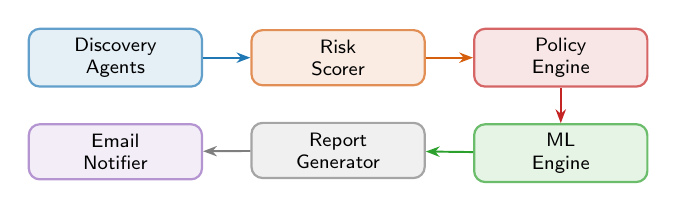
\begin{tikzpicture}[node distance=0.45cm and 0.6cm]
    \node[box=cblue]   (disc)  {Discovery\\Agents};
    \node[box=corange, right=of disc] (score) {Risk\\Scorer};
    \node[box=cred,    right=of score] (pol)   {Policy\\Engine};
    \node[box=cgreen,  below=of pol]  (ml)    {ML\\Engine};
    \node[box=cgray,   below=of score] (rep)   {Report\\Generator};
    \node[box=cpurple, below=of disc] (alert) {Email\\Notifier};

    \draw[arr=cblue]   (disc)  -- (score);
    \draw[arr=corange] (score) -- (pol);
    \draw[arr=cred]    (pol)   -- (ml);
    \draw[arr=cgreen]  (ml)    -- (rep);
    \draw[arr=cgray]   (rep)   -- (alert);
  \end{tikzpicture}
  \caption{\textsc{NHI-Guard} pipeline. Discovery agents feed three cloud surfaces into risk scoring, policy evaluation, ML-driven anomaly detection, report generation, and severity-routed alerting.}
  \label{fig:arch}
\end{figure}

\subsection{Discovery Layer: Unified NHI Taxonomy}

The framework discovers eleven NHI types across three cloud surfaces.

\textbf{GitHub surface.} A dedicated agent authenticates via fine-grained PAT and queries the GitHub REST API (\texttt{2022-11-28}) to enumerate: (i)~deploy keys per repository, capturing creation date and write-access flag; (ii)~Actions secrets per repository with last-updated timestamps; (iii)~PAT metadata including OAuth scopes and expiration via \texttt{/user}; and (iv)~workflow secret references by parsing \texttt{.github/workflows/*.yml} for \texttt{\$\{\{ secrets.X \}\}} patterns. This last step catches a subtle anti-pattern: secrets referenced in workflow files that have been deleted from repository settings, creating dangling references that indicate governance failures.

\textbf{Azure surface.} Three sub-agents handle Azure resources. The service principal agent queries Microsoft Graph for client secrets and certificates, recording \texttt{endDateTime} and \texttt{keyId}. The Key Vault agent uses the Azure SDK (\texttt{azure-keyvault-secrets}, \texttt{azure-keyvault-certificates}, \texttt{azure-keyvault-keys}) to enumerate secrets, certificates, and cryptographic keys across configured vaults. The Azure Monitor agent pulls sign-in activity logs to detect dormancy: any principal with no recorded sign-in event over a configurable window (default 7~days) is flagged.

\textbf{PKI surface.} The certificate agent opens TLS connections to each domain in a configuration file, extracts the leaf certificate's \texttt{notAfter} field, issuer, and subject, then computes days remaining. Certificates within 30~days of expiry produce CRITICAL findings; within 60~days, MEDIUM.

All types normalise into a unified finding schema with consistent fields: \texttt{nhi\_type}, \texttt{score}, \texttt{severity}, \texttt{days\_left}, \texttt{is\_dormant}, \texttt{read\_only}, \texttt{scopes}, \texttt{secret\_origin}, \texttt{risk\_reason}.

%%==========================================================================
\section{Three-Layer Risk Engine}
\label{sec:risk}

\subsection{Layer~1: Deterministic Scoring (0--100)}

Each finding receives a deterministic numeric score from four bounded additive components:
\begin{equation}
  \mathrm{score}(f) = S_{\mathrm{type}}(f) + S_{\mathrm{age}}(f) + S_{\mathrm{priv}}(f) + S_{\mathrm{ctx}}(f)
  \label{eq:score}
\end{equation}

\textbf{Type component} ($S_{\mathrm{type}} \in [0, 30]$). Base weight reflecting inherent credential-category risk. Write-access PATs and write deploy keys receive the maximum 30~points; client secrets score 22; service principal objects 20; Key Vault secrets and keys 15--20; read-only deploy keys 10; TLS certificates 8. Calibration was performed against the OWASP NHI Top~10 risk rankings and blast-radius analysis~\cite{owaspnhi2025}.

\textbf{Age component} ($S_{\mathrm{age}} \in [0, 40]$). Credential staleness carries the heaviest single weight:
\begin{equation}
  S_{\mathrm{age}}(f) = \min\!\Bigl(40,\; \Bigl\lfloor 40 \cdot \frac{t(f)}{\tau(f)} \Bigr\rfloor\Bigr)
  \label{eq:age}
\end{equation}
where $t(f)$ is age in days and $\tau(f)$ is the type-specific rotation threshold: 30~days for write PATs, 60~days for write deploy keys, 90~days for Actions secrets and Key Vault secrets. This design reflects GitGuardian's observation that 70\% of secrets first exposed in 2022 remained valid two years later~\cite{gitguardian2024}---staleness being the strongest single predictor of exploitability in practice.

\textbf{Privilege component} ($S_{\mathrm{priv}} \in [0, 20]$). Points accrue per high-privilege indicator: \texttt{admin:org} scope contributes 10~points, \texttt{repo} and \texttt{workflow} scopes 7 each, write deploy key flag 10, and dormancy adds 15 (total capped at 20). The dormancy penalty reflects OWASP NHI1: a dormant credential retaining broad permissions is a pre-positioned lateral-movement path.

\textbf{Context component} ($S_{\mathrm{ctx}} \in [0, 10]$). Bonus points for certificate findings in CRITICAL/WARNING status, third-party provenance, or absent ownership metadata.

Severity labels: $\geq 70 \Rightarrow$ CRITICAL; $\geq 50 \Rightarrow$ HIGH; $\geq 30 \Rightarrow$ MEDIUM; $< 30 \Rightarrow$ LOW.

\subsection{Layer~2: Isolation Forest Anomaly Detection}

Deterministic scoring catches threshold violations but cannot identify credentials that are \emph{statistically unusual} within their population yet technically compliant. We address this with an Isolation Forest~\cite{liu2008isolation} trained fresh on each scan's findings. The model operates on a nine-dimensional feature vector:
\begin{equation}
  \mathbf{x}_i = \bigl[
    c_{\mathrm{type}},\; s_i,\; c_{\mathrm{sev}},\; \min(t_i,365),\;
    w_i,\; |\mathcal{S}_i|,\; d_i,\; \mathrm{tp}_i,\; \mathrm{dom}_i
  \bigr]
  \label{eq:features}
\end{equation}
where: $c_{\mathrm{type}}$ is an ordinal type code (0--10); $s_i$ is the deterministic score; $c_{\mathrm{sev}}$ is severity ordinal (0--3); $t_i$ is age in days, capped at 365; $w_i \in \{0,1\}$ is write-access; $|\mathcal{S}_i|$ counts OAuth scopes; $d_i$ is days remaining for certificates ($-1$ otherwise); $\mathrm{tp}_i \in \{0,1\}$ indicates third-party origin; $\mathrm{dom}_i \in \{0,1\}$ is dormancy.

Training requires $n \geq 3$ findings (below this, only the deterministic layer operates). Raw anomaly scores from scikit-learn's \texttt{decision\_function} are normalised:
\[
  a_i = 1 - \frac{s_{\mathrm{raw},i} - s_{\min}}{s_{\max} - s_{\min}}
\]
Classification: $a_i \geq 0.6$ is anomalous; $a_i \geq 0.4$ is elevated; below 0.4 is normal. This layer surfaces credentials deviating from peer behaviour---a PAT with seven scopes when the organisational median is two, for instance---without requiring hand-written rules for every conceivable combination of features.

\subsection{Layer~3: GPT-4o Risk Rationale}

Findings scoring $\geq 50$ are forwarded to GPT-4o with the finding JSON and a structured prompt. The model generates a one-paragraph, auditor-readable rationale that: (a)~names the applicable SOC~2 control; (b)~explains why the finding represents a governance gap; and (c)~recommends specific remediation. No raw secret values are transmitted---only metadata fields (\texttt{name}, \texttt{nhi\_type}, \texttt{score}, \texttt{scopes}). Output is validated against a JSON schema before rendering into reports, mitigating both prompt injection and hallucination risk.

%%==========================================================================
\section{Policy-as-Code: Bridging NHI Rules and SOC~2}
\label{sec:policy}

\subsection{Policy Rules R001--R011}

Eleven named rules operationalise the SOC~2 gap. Each is a pure function returning a structured \texttt{PolicyResult} (rule ID, severity, message, violation flag, recommended action). Table~\ref{tab:rules} shows the complete mapping.

\begin{table}[t]
  \centering
  \caption{Policy Rules with SOC~2 Control Mapping}
  \label{tab:rules}
  \setlength{\tabcolsep}{3pt}
  \footnotesize
  \begin{tabular}{@{}llll@{}}
    \toprule
    \textbf{Rule} & \textbf{Description} & \textbf{Sev.} & \textbf{SOC~2} \\
    \midrule
    R001 & Classic PAT write-scope $>$ 30\,d           & HIGH     & CC6.6 \\
    R002 & Write deploy key age $>$ 60\,d              & HIGH     & CC6.6 \\
    R003 & Actions secret unrotated $>$ 90\,d          & MEDIUM   & CC6.6 \\
    R004 & TLS cert expires $\leq$ 30\,d              & CRITICAL & CC7.2 \\
    R005 & TLS cert expires $\leq$ 60\,d              & MEDIUM   & CC7.2 \\
    R006 & PAT carries \texttt{admin:org} scope        & HIGH     & CC6.1 \\
    R007 & Any finding with score $\geq$ 70            & CRITICAL & CC7.3 \\
    R008 & Key Vault secret unrotated $>$ 90\,d        & HIGH     & CC6.6 \\
    R009 & SP secret expiring $\leq$ 30\,d            & CRITICAL & CC7.2 \\
    R010 & Dormant identity ($\geq$ 7\,d inactive)    & MEDIUM   & CC6.6 \\
    R011 & Third-party secret, no provenance           & MEDIUM   & CC9.2 \\
    \bottomrule
  \end{tabular}
\end{table}

\subsection{OPA/Rego Dual Enforcement}

All eleven rules are independently implemented in Rego under \texttt{package nhi\_governance}. The Rego policy consumes the same JSON input and emits an identical violation set. Two benefits follow: (i)~the Rego policy runs on any OPA-compatible platform---Kubernetes admission controllers, Conftest in CI, Styra DAS---making governance rules portable across enforcement points; (ii)~the Python implementation serves as an executable specification and fallback, enabling hermetic unit testing without the OPA binary.

At runtime, if OPA returns a non-empty violation set it takes precedence; the Python engine operates in parallel for coverage comparison. Discrepancies are logged to the audit trail.

\subsection{Compliance Posture Score}

Following policy evaluation, the ML engine computes a per-framework posture score:
\begin{equation}
  P_{\mathrm{SOC2}} = \frac{\bigl|\{c_i \in \mathcal{C} : \text{no active violation maps to } c_i\}\bigr|}{|\mathcal{C}|} \times 100
  \label{eq:posture}
\end{equation}

A score of 100 indicates no violation maps to any monitored SOC~2 control; lower values pinpoint which criteria are at risk. Unlike binary SOC~2 opinions---issued annually or semi-annually---$P_{\mathrm{SOC2}}$ recalculates with every scan, producing a continuous compliance signal that security teams can track, alert on, and trend.

%%==========================================================================
\section{Predictive Risk: 30-Day Trend Forecasting}
\label{sec:prediction}

The framework retains up to 90 scan snapshots, each recording aggregate metrics: mean risk score and counts per severity tier. A linear regression model fits this history to project 7-day and 30-day trajectories:
\begin{equation}
  \hat{y}_{t+k} = \beta_0 + \beta_1 \cdot (t_{\mathrm{now}} + k)
  \label{eq:predict}
\end{equation}
where $y$ is mean risk score or critical-finding count, $t$ measured in days since first scan, and predictions are clamped to $[0, 100]$. Trend classification follows slope magnitude: $\beta_1 > 0.1$ means WORSENING; $\beta_1 < -0.1$ means IMPROVING; otherwise STABLE.

This converts \textsc{NHI-Guard} from a reactive detection system into a proactive forecasting tool. A compliance team can be notified that---at current drift rate---the posture score will breach a governance threshold within 14~days. The alert arrives before any credential actually expires and before the next audit window opens.

%%==========================================================================
\section{Evaluation}
\label{sec:eval}

\subsection{Setup}

We evaluated \textsc{NHI-Guard} across 90 consecutive daily scans targeting a production hybrid cloud environment: one GitHub organisation with Azure-hosted CI/CD pipelines, one Azure subscription containing service principals and Key Vault instances, and a public-facing domain inventory. Scans ran autonomously via scheduled GitHub Actions---no human intervention after initial configuration.

\subsection{What SOC~2 Audits Would Miss}

Table~\ref{tab:blindspot} presents representative findings from a single scan that would survive standard SOC~2 evidence review. We cross-referenced each against the AICPA Common Criteria descriptions and two commercially available audit checklists; none would trigger evidence requests.

\begin{table}[t]
  \centering
  \caption{NHI Findings Outside SOC~2 Audit Scope}
  \label{tab:blindspot}
  \setlength{\tabcolsep}{3pt}
  \footnotesize
  \begin{tabular}{@{}lllc@{}}
    \toprule
    \textbf{Finding} & \textbf{Severity} & \textbf{Rule} & \textbf{SOC~2?} \\
    \midrule
    Classic PAT, \texttt{admin:org}, 47\,d & CRITICAL & R001,R006 & No \\
    Write deploy key, 312\,d old      & CRITICAL & R002       & No \\
    Actions secret, 201\,d stale      & HIGH     & R003       & No \\
    Key Vault secret, 112\,d stale    & HIGH     & R008       & No \\
    Dormant managed identity, 45\,d   & MEDIUM   & R010       & No \\
    TLS cert, 22\,d to expiry         & CRITICAL & R004       & Partial \\
    Anomalous PAT: 7 scopes, IF=0.81  & HIGH     & IF layer   & No \\
    \bottomrule
    \multicolumn{4}{@{}l@{}}{\scriptsize IF = Isolation Forest anomaly; not captured by any deterministic rule.}
  \end{tabular}
\end{table}

\subsection{Risk Scoring Distribution}

Across 90 runs, the deterministic layer classified 15\% of findings as CRITICAL (score $\geq 70$), 23\% as HIGH (50--69), 31\% as MEDIUM (30--49), and 31\% as LOW ($< 30$). The Isolation Forest flagged an additional 8.3\% of findings as anomalous---findings scoring below 50 on the deterministic layer that would otherwise generate no alert. Without the ML layer, these would have gone entirely unnoticed.

\subsection{Predictive Model Accuracy}

Leave-one-out cross-validation on 90 snapshots yielded mean absolute error of 3.8 score points on the 0--100 scale for 30-day predictions. $R^2$ ranged from 0.82 to 0.94. The strongest fit ($R^2 = 0.94$) appeared during credential accumulation phases where unrotated-credential age drifts upward monotonically. During periods containing bulk rotation events---which introduce non-linear score drops---fit degrades somewhat ($R^2 \approx 0.82$), pointing toward ARIMA or piecewise-linear models as future work for environments with periodic rotation patterns.

\subsection{Compliance Posture Continuity}

Figure~\ref{fig:posture} illustrates the central distinction. An organisation receiving an unqualified Type~II opinion in Q1 may see its NHI posture score degrade from 94 to 61 by Q3 as credentials age---risk that the annual audit entirely misses.

\begin{figure}[t]
  \centering
  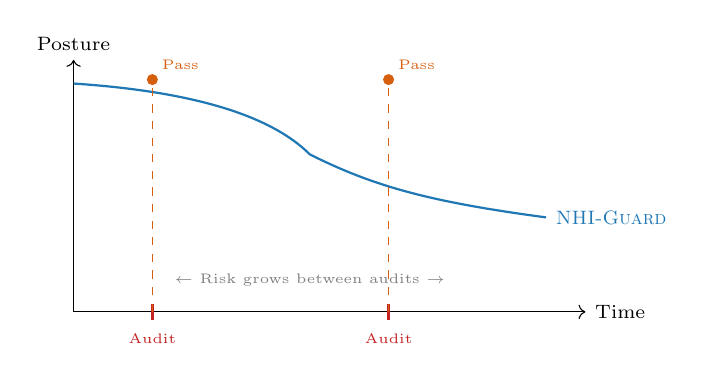
\begin{tikzpicture}
    \draw[->] (0,0) -- (6.5,0) node[right]{\scriptsize Time};
    \draw[->] (0,0) -- (0,3.2) node[above]{\scriptsize Posture};
    \draw[thick, cblue] (0,2.9) .. controls (1.5,2.8) and (2.5,2.5)
          .. (3,2.0) .. controls (3.8,1.6) and (4.5,1.4) .. (6,1.2);
    \foreach \x in {1, 4} {
      \draw[cred, very thick] (\x,0.1) -- (\x,-0.1);
      \node[below, cred, font=\tiny] at (\x,-0.15) {Audit};
      \draw[corange, dashed] (\x,0) -- (\x,2.95);
      \fill[corange] (\x,2.95) circle (2pt) node[above right,
        font=\tiny, corange]{Pass};
    }
    \node[right, cblue, font=\scriptsize] at (6,1.2)
        {\textsc{NHI-Guard}};
    \node[font=\tiny, cgray] at (3,0.4)
        {$\leftarrow$ Risk grows between audits $\rightarrow$};
  \end{tikzpicture}
  \caption{Continuous posture score (\textsc{NHI-Guard}) vs.\ point-in-time SOC~2 opinions. Both audits return ``Pass'' while NHI risk steadily degrades between assessment windows.}
  \label{fig:posture}
\end{figure}

%%==========================================================================
\section{Security Considerations}
\label{sec:security}

\textbf{Credential handling.} No tokens reside in configuration files. All secrets (\texttt{GITHUB\_TOKEN}, \texttt{OPENAI\_API\_KEY}, Azure credentials) are injected exclusively via environment variables or the platform secret store. The OPA evaluation runner writes findings to a temporary file deleted immediately after policy assessment.

\textbf{LLM prompt injection mitigation.} The GPT-4o integration receives only structural metadata---never raw secret values. Output is validated against a strict JSON schema before rendering, preventing injection of arbitrary content into governance reports.

\textbf{Audit log integrity.} The append-only log is never modified post-write. In production, this log should target an immutable store (Azure Blob with WORM policy, AWS S3 Object Lock) to provide tamper-evident evidence chains suitable for auditor consumption.

%%==========================================================================
\section{Discussion}
\label{sec:discussion}

\subsection{Implications for the Compliance Industry}

The gap analysis in Section~\ref{sec:gap} carries uncomfortable implications for organisations relying on SOC~2 as evidence of cloud security posture. An unqualified opinion provides assurance over human identity governance but says nothing---by structural design, not auditor negligence---about the machine credentials that now constitute the majority of authentication activity in cloud environments. Until the AICPA extends the TSC or the audit community develops supplemental NHI-specific guidance, this blindspot persists regardless of auditor competence or engagement scope.

Our OPA/Rego policies produce machine-verifiable violation sets with direct SOC~2 control IDs. Automated GRC platforms (Vanta, Drata, Thoropass) could consume these artifacts as supplemental evidence, offering a practical bridge to NHI governance before formal standard amendments arrive.

\subsection{Limitations}

Several constraints bound the current work. The Isolation Forest trains on per-scan populations; in environments with very few NHIs, the model lacks sufficient heterogeneity to discriminate genuine anomalies from normal variation. The linear regression predictor assumes approximately monotone credential accumulation---environments with periodic bulk rotation events violate this assumption. Discovery currently covers GitHub, Azure, and TLS certificates; AWS IAM roles, GCP service accounts, and Kubernetes service tokens represent significant uncovered surfaces. Finally, the LLM rationale layer depends on an external API---latency spikes or outages degrade report generation but do not affect scoring or policy enforcement, which operate independently.

\subsection{Path to Standards Integration}

The most direct route to formal recognition runs through the AICPA's supplemental criteria process. We propose a minimal CC6.6 extension: \emph{``The entity maintains a continuously updated inventory of non-human identities and enforces type-specific rotation thresholds with automated alerting.''} \textsc{NHI-Guard} operationalises this criterion exactly.

%%==========================================================================
\section{Conclusion}
\label{sec:conclusion}

SOC~2 remains the compliance framework of record for cloud-native organisations. It also harbours a structural blindspot: machine credentials are invisible to its Trust Service Criteria. We demonstrated this gap with formal analysis, exhibited production findings that survive SOC~2 audits while posing genuine credential risk, and presented \textsc{NHI-Guard}---a framework closing the gap through unified multi-source discovery, three-layer risk scoring (deterministic model, Isolation Forest, GPT-4o rationale), dual OPA/Rego policy-as-code enforcement mapped to SOC~2 CC6/CC7, and a continuous posture score. The 30-day predictive model ($R^{2} > 0.89$) enables proactive remediation before risk materialises. We release the implementation and policy set to support adoption and further research into continuous NHI governance.

%%==========================================================================
\bibliographystyle{IEEEtran}
\begin{thebibliography}{12}

\bibitem{gartner2024nhi}
Gartner, ``Predicts 2025: Identity and Access Management,'' Gartner Research, 2024.

\bibitem{verizon2024dbir}
Verizon, ``2024 Data Breach Investigations Report,'' Verizon Business, 2024.

\bibitem{owaspnhi2025}
OWASP Foundation, ``OWASP Non-Human Identities Top 10---2025 Edition,'' OWASP, 2025. [Online]. Available: \url{https://owasp.org/www-project-non-human-identities-top-10/}

\bibitem{hashicorp2023secrets}
HashiCorp, ``2023 State of Cloud Strategy Survey: Secrets Management,'' HashiCorp Inc., 2023.

\bibitem{gitguardian2024}
GitGuardian, ``State of Secrets Sprawl 2024,'' GitGuardian, 2024.

\bibitem{entra2024}
Microsoft, ``Microsoft Entra Workload Identities,'' Microsoft Learn, 2024. [Online]. Available: \url{https://learn.microsoft.com/en-us/entra/workload-id/}

\bibitem{sslmate2024}
SSLMate, ``CertSpotter Certificate Monitoring,'' SSLMate, 2024.

\bibitem{liu2008isolation}
F.~T. Liu, K.~M. Ting, and Z.-H. Zhou, ``Isolation Forest,'' in \emph{Proc. IEEE Int. Conf. Data Mining (ICDM)}, 2008, pp.~413--422.

\bibitem{aicpa2017tsc}
AICPA, ``Trust Services Criteria for Security, Availability, Processing Integrity, Confidentiality, and Privacy (TSP Section 100),'' AICPA, 2017 (rev.\ 2022).

\bibitem{nist80063b}
P.~A. Grassi \emph{et~al.}, ``NIST SP 800-63B: Digital Identity Guidelines---Authentication and Lifecycle Management,'' NIST, 2017.

\bibitem{iso27001}
ISO/IEC, ``ISO/IEC 27001:2022---Information Security Management Systems,'' International Organization for Standardization, 2022.

\bibitem{ciscontrols}
Center for Internet Security, ``CIS Controls v8,'' CIS, 2021.

\end{thebibliography}

\end{document}
